\section{Hysteretic neural networks\label{sec:chapter3:hnn}}
\subsection{Play and Prandtl-Ishlinskii networkds\label{sec:chapter3:play-and-pi-networks}}
\\
Consider $K > 0$ play operators. Each of them maps an initial state $p_{0}^{k} \in \mathbb{R} $ and an input sequence $x_1, x_2, \ldots$ to an output sequence $p_{1}^{k}, p_{2}^{k}, \ldots \ $, i.e.,

% \begin{equation}\label{eqn:input_to_op_output_mapping}
\begin{equation*}
  p_{0}^{k}, (x_1, x_2, \ldots) \mapsto (p_{1}^{k}, p_{2}^{k}, \ldots), k = 1, \ldots, K
\end{equation*}

The $k$th play operator is given by:

\begin{equation}\label{\eqn:chapter3:play-operator}
  p_{n}^{k} = G(x_{n}, p_{n-1}^{k}, w^{k}) := p_{n-1}^{k} + \Phi(w^{k} x_{n} - p_{n-1}^{k}), n = 1, 2, \ldots
\end{equation}

where $w^{k}$ are parameters and

\begin{equation}\label{\eqn:chapter3:phi}
  \begin{aligned*}
    \Phi(x) =
    \begin{cases}
      x - \frac{1}{2}, & x > \frac{1}{2} \\
      0,               & -\frac{1}{2} <= x <= \frac{1}{2} \\
      x + \frac{1}{2}, & x < \frac{1}{2}
    \end{cases}
  \end{aligned*}
\end{equation}

See Fig. \ref{fig:chapter3:phi}

\begin{figure}[htb]
  \centering
  \resizebox{8cm}{!}{\documentclass{standalone}
\usepackage{tikz}
\begin{document}
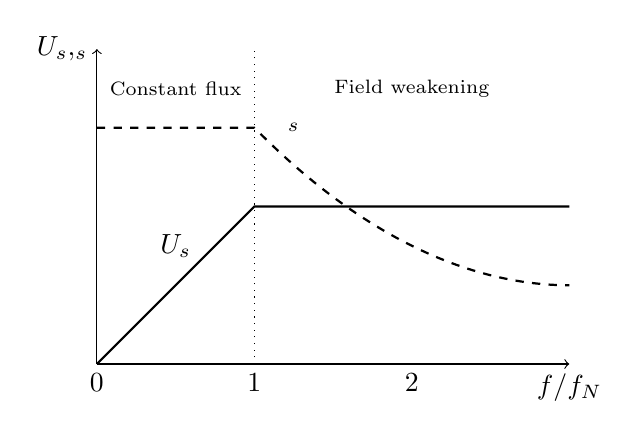
\begin{tikzpicture}
% horizontal axis
\draw[->] (0,0) -- (6,0) node[anchor=north] {$f/f_N$};
% labels
\draw	(0,0) node[anchor=north] {0}
		(2,0) node[anchor=north] {1}
		(4,0) node[anchor=north] {2};
% ranges
\draw	(1,3.5) node{{\scriptsize Constant flux}}
		(4,3.5) node{{\scriptsize Field weakening}};

% vertical axis
\draw[->] (0,0) -- (0,4) node[anchor=east] {$U_s,\varPsi_s$};
% nominal speed
\draw[dotted] (2,0) -- (2,4);

% Us
\draw[thick] (0,0) -- (2,2) -- (6,2);
\draw (1,1.5) node {$U_s$}; %label

% Psis
\draw[thick,dashed] (0,3) -- (2,3) parabola[bend at end] (6,1);
\draw (2.5,3) node {$\varPsi_s$}; %label

\end{tikzpicture}
\end{document}
}
  \caption{$\Phi(x)$}\label{fig:chapter3:phi}
\end{figure}

It can be represented as a recurrent neural network, see Fig. \ref{fig:chapter3:phi}. Note that in such a form the network is not feed-forward.
One can unfold it to make it feed-forwaard, see Fig. \ref{fig:chapater3:play-operator}

\theoremstyle{definition}
\begin{definition}
We call this network a \textsl{play network}. If there are \textsl{m} elements in the sequence ${x_n}$, we say the unfolded network is \textsl{m-unfolded}
\end{definition}

For example, the network in Fig. \ref{fig:chapter3:unfolded-nn} is 2-unfolded.
